The Python package plotly \cite{plotly} is used to display the network. Usually this package allows for the creation of figures that are then displayed in Jupyter notebooks, an extra window or saved as PNGs. However, if only plotly is used, there is no way to edit a created figure without completely regenerating it, which would then open a new window that displays the figure. For the use case of this app, the figures must be able to be updated within the same window so the simulation and different settings for viewing the networks are possible.

To accomplish this, the figures plotly creates can be hosted on a webserver, which is then able to update the network that the website displays. Plotly offers a built-in website framework called dash. The dash app is created using the statement in listing \ref{lst:dash_app}. The CSS of the website uses the dash bootstrap CSS as a base and font awesome \cite{fontAwesome} is used for the icons. The assets folder is set because the website uses some custom CSS located in that folder, that overrides some of the default dash bootstrap CSS.

\begin{lstlisting}[language=python, caption={Instatiate a new Dash app}, label={lst:dash_app}]
app = Dash(
    external_stylesheets=[dbc.themes.BOOTSTRAP, dbc.icons.FONT_AWESOME],
    assets_folder=os.getcwd() + "/assets",
    suppress_callback_exceptions=True,
)
app.layout = dash.html.div(id="page-content")
app.run()
\end{lstlisting}

After calling \texttt{app.run()}, this app automatically starts a flask server that hosts the website at \texttt{http://localhost:8050}. To specify what the website displays, the \texttt{layout} property of the \texttt{app} is set to the desired HTML components. Plotly provides HTML components as Python classes as well as some custom bootstrap components that are more advanced HTML elements like a sidebar. In this case, a simple div with the id \texttt{page-content} is used. The children of this div are then changed depending on which page needs to be displayed.

The webapp consists of three different pages:
\begin{itemize}
    \item \textbf{View}: Displays a 3D network and offers some controls to alter the appearance
    \item \textbf{Simulation}: Displays the same network as the view does with the same controls and offers functionality to run the simulation in that network.
    \item \textbf{Stats}: Shows stats collected during the simulation with controls for which 
    stats to display
\end{itemize}

To change between these pages, three routes are created for the app so each page has its own URL: \texttt{/view}, \texttt{/sim} and \texttt{/stats}. To display the correct page for each URL, a callback is used to change the content of the \texttt{page-content} div. This callback is invoked whenever any URL of the webserver is accessed, it is shown in listing \ref{lst:page_content}.
\begin{lstlisting}[language=python, caption={Create callback for page content}, label={lst:page_content}]
@callback(
            Output("page-content", "children"),
            [Input("url", "pathname")],
)
def display_page(pathname):
    if pathname == "/view":
        html_view.reset()
        return html_view.layout
    elif pathname == "/sim":
        sim_view.reset()
        return sim_view.layout
    elif pathname == "/stats":
        stats_view.reset()
        return stats_view.layout
    else:  # if redirected to unknown link
        return "404"
\end{lstlisting}

\section{Network View}
The website for the network view consists of a collapsible sidebar on the left that provides the controls for the appearance of the network. The rest of the page is used to display the network. Figure \ref{fig:web_network_view} depicts the UI of this page.

\begin{figure}
    \centering
    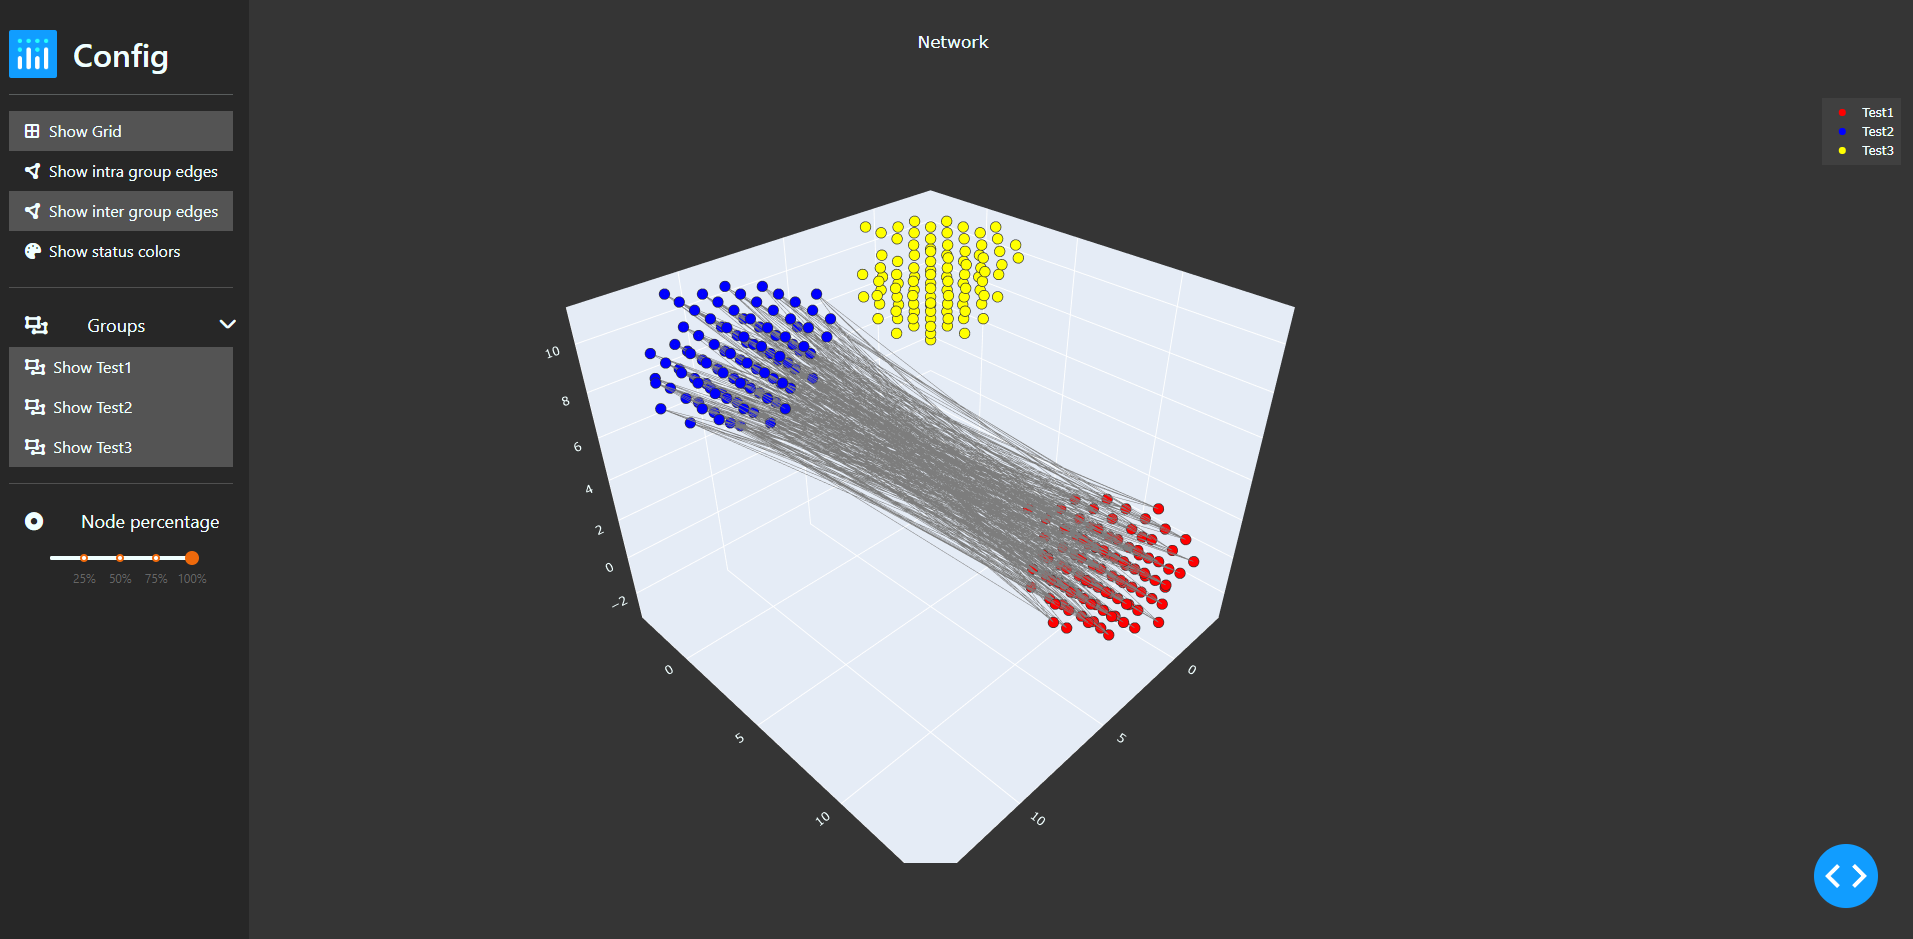
\includegraphics[width=0.5\linewidth]{images/web_network_view.png}
    \caption{UI for the network view webpage}
    \label{fig:web_network_view}
\end{figure}

The sidebar contains buttons to visually disable or enable the grid, intra/inter group edges, group/status color or groups of nodes. The slider can be used to reduce the number of displayed nodes, which can help to improve performance for large networks. Each of these settings uses a callback to update the network. Listing \ref{lst:grid_callback} contains such a callback for toggling the grid. This callback updates the style of the button to change the background color, depending on whether the button is now enabled or disabled. The \texttt{update\_graph\_grid} edits the necessary settings in the plotly figure to enable or disable the grid and then returns the updated figure. The two return values of the \texttt{toggle\_grid} function are passed to the specified outputs, which contain the UI element ids for the button and network figure. By using these outputs, dash ensures that the changes are reflected on the website without having to reload it. Similar callbacks are created for the other buttons and the slider.

\begin{lstlisting}[language=python, caption={Callback for toggling the grid}, label={lst:grid_callback}]
@callback(
    [
        Output(self.id_factory("grid-button"), "style"),
        Output(self.id_factory("live-graph"), "figure", allow_duplicate=True),
    ],
    [Input(self.id_factory("grid-button"), "n_clicks")],
    prevent_initial_call=True,
)
def toggle_grid(_):
    self.sidebar.show_grid = not self.sidebar.show_grid
    return {
        "background-color": self.ENABLED_COLOR
        if self.sidebar.show_grid
        else self.BACKGROUND_COLOR
    }, self.update_graph_grid(self.sidebar.show_grid)
\end{lstlisting}

The plotly figure for the network, which makes up the rest of the webpage, offers some controls for viewing the 3D network. The camera can be rotated by holding down the left mouse button or moved by holding down the right mouse button. The zoom can be changed with the mouse wheel and in the top right corner there are buttons for these controls as well as a button to download the current view as a PNG. Chapter \ref{cha:network_display} explains how the network figure is created.

\section{Simulation view}
The simulation view contains the same UI as the network view. Its class inherits from the network view. Then 5 new buttons are added to control the simulation: reset simulation, show log output, advance one step, enable auto advancing (1 step per second) and save statistics. Using these five buttons as well as the sidebar to control the appearance of the network, the simulation can be run, updating the graph with new colors for the current state of each node after each step. This is done in the callback of the advance step button, as shown in listing \ref{lst:step_callback}, which executes one simulation step and then computes the new color sequence and log output. The updated graph and log console text are then returned to the outputs to update the website.

\begin{lstlisting}[language=python, caption={Callback for advancing simulaton by one step}, label={lst:step_callback}]
@callback(
    Output(self.id_factory("live-graph"), "figure", allow_duplicate=True),
    Output("log-console-content", "children", allow_duplicate=True),
    Input(self.id_factory("step"), "n_clicks"),
    prevent_initial_call=True,
)
def step(_):
    with self.sim_mutex:
        self.sim.simulate_step()
        color_map, _ = self.sim.create_color_seq()
        if self.show_logs:
            return (
                self.graph.update_status_colors(color_map),
                self.sim.stats.get_log_text_html(),
            )
        else:
            return self.graph.update_status_colors(color_map), ""
\end{lstlisting}

The reset button opens a popup that requires confirmation from the user before the simulation is  reset. The save button also opens a popup that allows the user to enter a name for the statistics of this simulation.

\section{Stats view}
The stats website displays statistics saved during simulations. When the website is opened for the first time, a popup window is displayed, allowing the user to select which statistics are to be displayed. This website contains a sidebar similar to the previous view and simulation pages. The sidebar contains buttons to control graphs for which statistics are displayed. The UI is shown in figure \ref{fig:web_stats_view}.

\begin{figure}
    \centering
    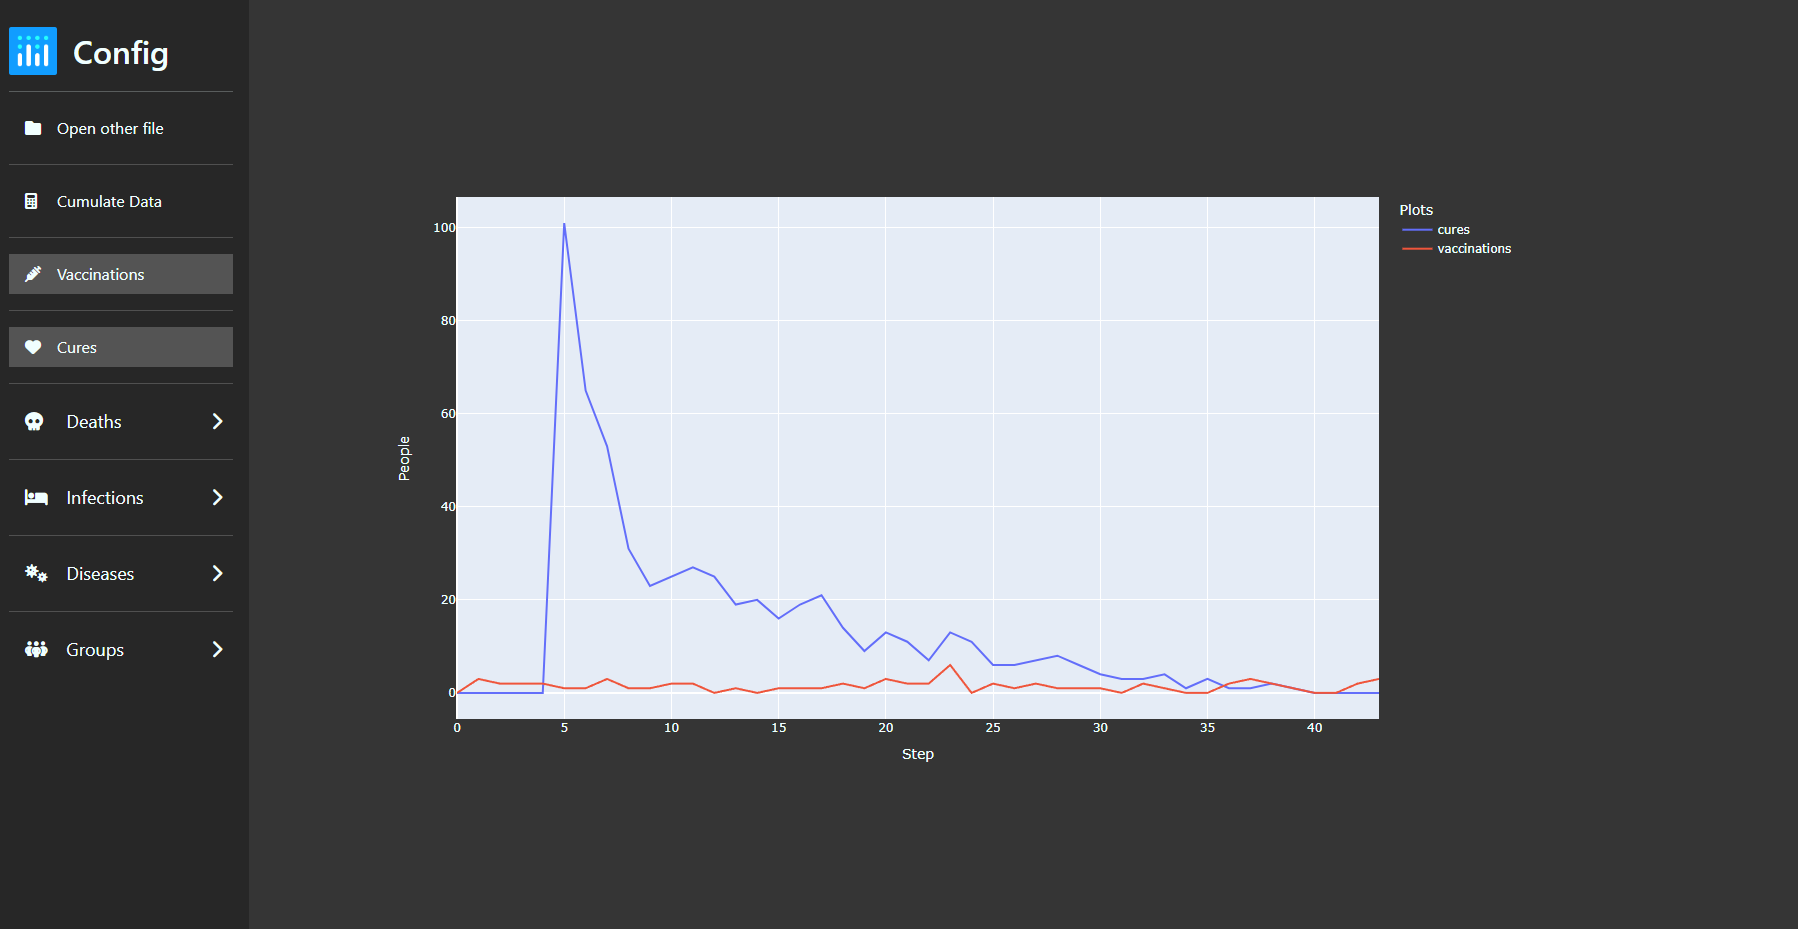
\includegraphics[width=0.5\linewidth]{images/web_stats_view.png}
    \caption{UI for the stats webpage}
    \label{fig:web_stats_view}
\end{figure}

The sidebar contains the following buttons:
\begin{itemize}
    \item Open another file: Brings the popup to select another stat file back up
    \item Cumulate data: Cumulates the graphs to show total up until each step instead of individual values of each step
    \item Display vaccinations, cures, deaths or infections data. Deaths and infections are split
    into total, vaccinated and unvaccinated
    \item Groups and diseases buttons allow to split the data to show only the values for a specific group/disease
    or the total for all diseases/groups
\end{itemize}
These buttons use callbacks to update the graphs similar to the ones for the network view.

\section{Updating the data}
Endpoints are created to update the network or available stats files that are displayed. The dash server allows the creation of listeners on URLs that are called when other applications send HTML POST requests to those URLs. To update the data, two endpoints are exposed, one for updating the network and one for updating the stat files. The creation of these endpoints is shown in listing \ref{lst:data_endpoints}. After a POST request is received, the JSON data it contains is decoded and stored for the stats or decoded, built and stored for networks. Then the view is reset to refresh all open webpages. Finally, a response is sent for either success (200) or failure (400).

\begin{lstlisting}[language=python, caption={Endpoints for updating data}, label={lst:data_endpoints}]
@app.server.route("/update-data", methods=["POST"])
def update():
    try:
        json_data = request.get_json()
        project.network = Network.from_dict(json_data)
        project.network.build()
        graph.update_network(project.network)
        html_view.reset()
        sim_view.reset()
        stats_view.reset()
        return make_response(jsonify({"status": "OK"}), 200)
    except Exception as e:
        return make_response(jsonify({"status": {str(e)}}), 400)

@app.server.route("/update-stats", methods=["POST"])
def update_stats():
    try:
        json_data = request.get_json()
        stats = SimStats.from_dict(json_data["stats"])
        project.stats[json_data["filename"]] = stats
        stats_view.reset()
        return make_response(jsonify({"status": "OK"}), 200)
    except Exception as e:
        return make_response(jsonify({"status": {str(e)}}), 400)
\end{lstlisting}
